\documentclass[a4paper,10pt,twoside,twocolumn]{dndbook} %a4, 10pt, book (idk why i did that...), 2 cols, dnd-themed
\usepackage[english]{babel} %language
\usepackage[utf8]{inputenc} %lovely utf-8
\usepackage{graphicx} %images
\usepackage{wrapfig} %images
\usepackage{array} %allways use this shit, idk why
\usepackage{tikz} %draw stuff
\usepackage{ifthen} %draw stuff
\usetikzlibrary{shapes,calc,fadings} %draw stuff
\usepackage{xspace} %usefull idk, allways import this stuff
\usepackage{dirtytalk} %\say because fuck it
\usepackage{setspace} %don't ask, kind of like it...
\usepackage{pgfplots}

\usepackage[singlelinecheck=false]{caption} %idk dndbook...
\usepackage{listings} %idk dndbook...
\usepackage{shortvrb} %not used yet...
\usepackage{stfloats} %idk dndbook
\usepackage{dirtytalk}

\singlespacing
\makeatletter %because of titlepage and \HUGE

\@openrightfalse %no empty pages

\graphicspath{ {./images/} }

\def \license {GNU Free Documentation License}
\def \licensetext {Please consider and respect the copyleft of this license. The content of this document should be accessible to everyone. Everyone has the right to use the content of this document as he/she wishes, to modify it, to publish it modified (taking into account the copyleft) and to republish it without any changes (taking into account the copyleft).}
\def \author {Sven Hugi}%if you edit this document, add your name... <3
\def \illustrators {} %add name
\def \othercontrib {} %add name

%highlighting with some random effect -> looks handmade and i love it...
\newcommand\hl[2][yellow]{
	\begin{tikzpicture}[
	baseline,
	decoration={random steps,amplitude=1pt,segment length=15pt},
	outer sep=-15pt, inner sep = 0pt
	]
	\node[decorate,rectangle,fill=#1,anchor=text]{#2\xspace};
	\end{tikzpicture}
}
%2 column layout hack...
\newcommand{\nextPage}{
	\newpage
	\hbox{}
	\newpage
}
%make bad things look ok...
\newcommand{\doublelinebreak}{
	\linebreak\linebreak
}
%the old HUGE fontsize
\newcommand\HUGE{\@setfontsize\Huge{60}{80}} 

\renewcommand{\maketitle}{
	\thispagestyle{empty}
	\onecolumn %fuck it
	\vspace*{5cm}
	\begin{center}
		$\vspace*{2cm}$
			{\HUGE\DndFontDropCap{KORRED}}\\	
	\end{center}
	\twocolumn %reset shit
}\makeatother

\begin{document}
	\maketitle
	\section*{Credits}
	\vspace{.25cm}
	\textbf{Authors:} \author\linebreak
	\textbf{Illustrators:} \illustrators\linebreak
	\textbf{Additional Contributors:} \othercontrib\linebreak
	\textbf{License:} \license\doublelinebreak
	\licensetext\doublelinebreak
	Inspiration from Volo's guide to monsters\linebreak
	Images from (I don't have the copyright):\linebreak
	https://forgottenrealms.fandom.com/wiki/Korred\linebreak
	https://www.pinterest.ch/pin/837599230697979097/
	\vfill\pagebreak\hbox{}\vfill\hfill{\tiny This Document was written in \LaTeX.}\pagebreak
	\section{Korred Traits}
	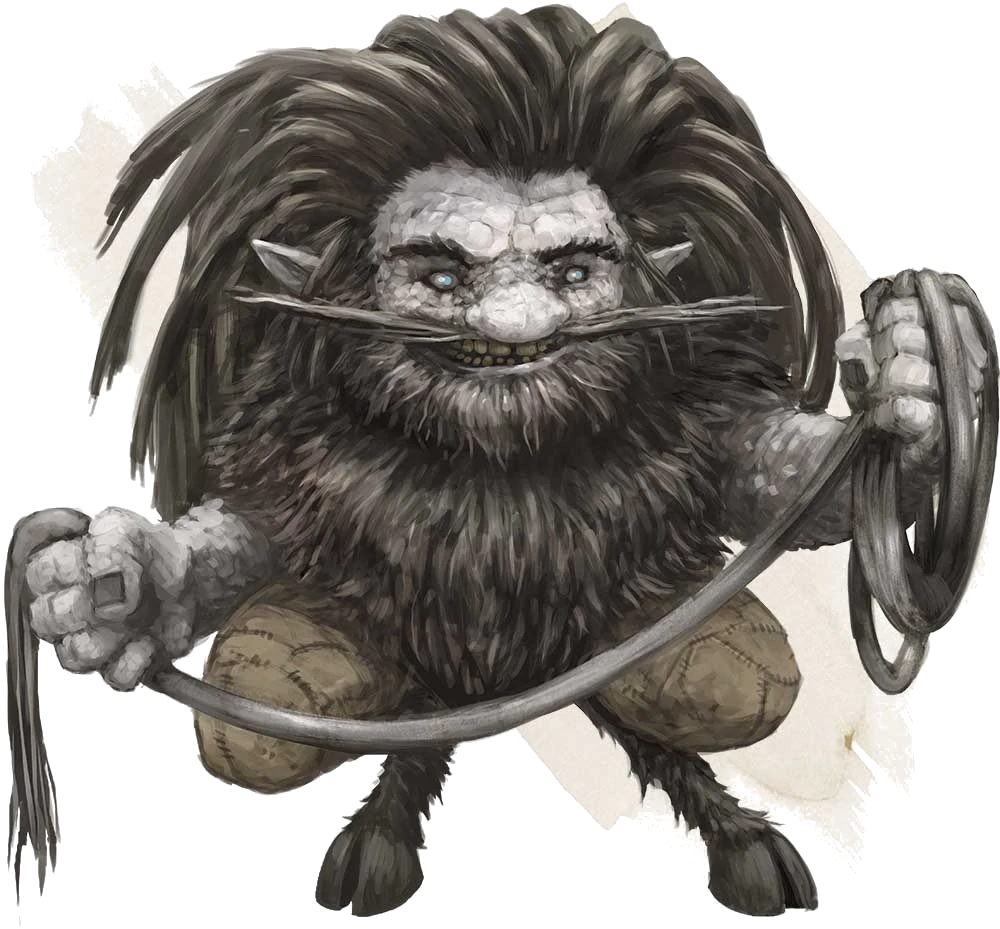
\includegraphics[width=\linewidth]{Korred5e.png}
	\textbf{Ability Score Increase.} Your Strength score increases by 2 and your Constitution score increases by 1.\linebreak
	\textbf{Age.} Korreds can live 500 years to almost 800 years. They reach adulthood at the age of 40.\linebreak
	\textbf{Alignment.} Korreds are unpredictable and secretive fey that prefer to keep their own company, typically fleeing from other creatures but becoming aggressive when feeling insulted or annoyed, especially when annoyed by the sound of mining. Korreds tend toward chaotic alignments. They are rarely evil and tend more towards neutral.\linebreak
	\textbf{Size.} Korreds stand around 4 feet tall and average about 250 pounds. Your size is Small.\linebreak
	\textbf{Speed.} Your base walking speed is 25ft. You have a burrow speed of 30ft even through stone. Swimming and Flying cost you an additional 1 extra foot of movement for every foot moved.\linebreak
	\textbf{Language.} Choose 2 between Common, Dwarvish, Gnomish, Sylvan, Terran, Undercommon\linebreak
	\textbf{Earthy Fey.} You are considered of the fey type.
	\textbf{Darkvision.} You can see in dim light within 60 ft of you as if it were bright light, and in darkness as if it were dim light. You can't discern color in darkness, only shades of gray.\linebreak
	\textbf{Stone's Strength.} While on ground made out of stone or dirt, you have a +2 bonus to damage rolls on your weapon attacks that use Strength, but if you aren't on the ground you have a -2 to damage rolls on your attacks.\linebreak
	\textbf{Stone Sympathy.} You can sense tunnels, passages and holes in the rock within 100 ft of you. You are also considered proficient in all Intelligence checks related to minerals. While touching the ground you can also feel every creature in a 120ft radius touching the ground (tremorsense).\vfill\pagebreak
	\textbf{Stone Camouflage.} You have advantage on Dexterity (Stealth) checks made to hide in rocky terrain.\linebreak
	\textbf{Enchanted Hair.} The hair that grows from your head is magical. You can manipulate the form of the cut hair and also use it as a rope (50ft). The rope has a ac of 17 and 20 hit points. Every round the rope regains 1 hit point while it has at least 1 hit point and you are not dead. If the rope drops to 0 hit points, it is destroyed. \linebreak
	\textbf{Command Hair.} You can use a action to command your hair to grapple a creature you can see in 15ft. The target must succeed on a Dexterity saving throw against your Wisdom score or becommes grappled. To escape the creature must succeed on a Strenght check against your Constitution score. You can use a bonus action to release the target. The target gets also released if you die or becomme incapacitated. The hair has a ac of 17 and 20 hit points. Every round the hair regains 1 hit point while it has at least 1 hit point and you are not dead. If the hair drops to 0 hit points, it gets cut and the target is released. You can use this feature a number of times equal to your Wisdome modifier in between long rests.
	\pagebreak
	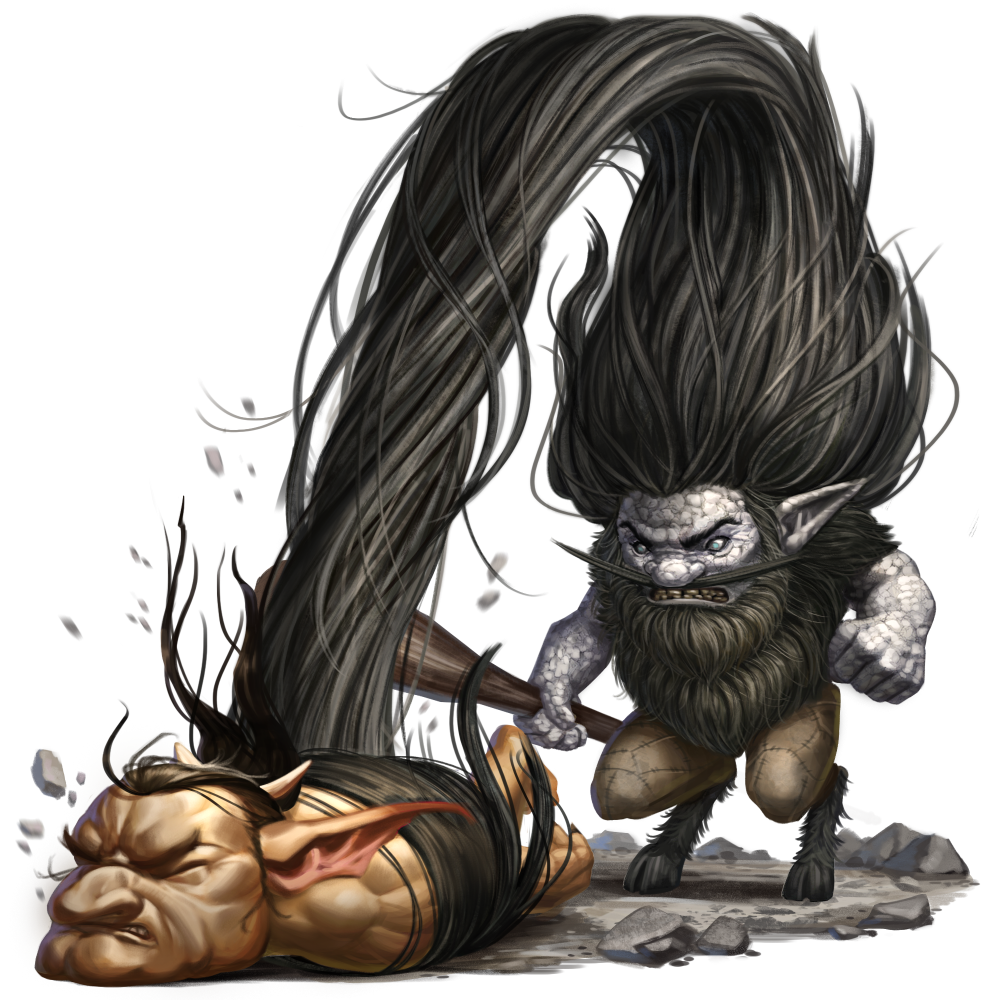
\includegraphics[width=\linewidth]{korred.png}

\end{document}